\documentclass[11pt,a4paper]{beamer}
\usepackage[ngerman]{babel}
\usepackage[T1]{fontenc}
\usepackage[utf8]{inputenc}
\usepackage{amsmath}
\usepackage{amsfonts}
\usepackage{amssymb}

% Notwendig für Gantt-Diagramme (Zeitstrahl)
\usepackage{tikz}
\usepackage{gantt}

\usetheme{Berlin}
\author{Julian Baumann, Xenia Kühling, Sebastian Ruder}
\title{Koreferenz mit BART}
\subtitle{Spezifikationsvortrag zum Softwareprojekt im Sommersemester 2014}
\date{27. Mai 2014}

\begin{document}
\maketitle

\section{Einführung}
\begin{frame}{Inhalt}
\tableofcontents
\end{frame}

\begin{frame}{Problematik: Koreferenz}
\begin{quote}

\textbf{John Simon}, \textbf{Chief Financial Officer of Prime Corp since 1986} saw \textbf{his} pay jump 20 percent, to 1.3 million dollar, as \textbf{the 37-year-old} also became \textbf{the financial service company’s president}.\footnote{Beispiele von Yannick Versley}
\end{quote}
\bigskip
\begin{itemize}
\item Unterschiedliche Beschreibungen beziehen sich auf gleiche Entitäten
\begin{itemize}
\item John Simon
\item he
\item the 37-year-old
\end{itemize}
\end{itemize}
\end{frame} 

\begin{frame}{Anwendungen: Information Extraction}
\begin{quote}


Towards the end of the war, under extreme pressure from the Nazi
Party, \textbf{Furtwängler} fled to Switzerland. [...]\\
\textbf{He} died in 1954 in Ebersteinburg close to Baden-Baden.
\end{quote}
\bigskip

\textbf{Q: Wann starb Furtwängler?}
\bigskip

$\rightarrow$ Wie kann man Koreferenz auflösen?




\end{frame}

\section{BART}
\begin{frame}{BART}
\begin{itemize}
\item Beautiful Anaphora Resolution Toolkit
\item Entstanden im Projekt\\ \textit{Exploiting Lexical and Encyclopedic Resources For Entity Disambiguation} 
im John Hopkins Summer Workshop 2007
\item System für automatische Koreferenzresolution
\item Weiterentwicklungen im Rahmen von shared tasks, für verschiedene Sprachen (Italienisch, Chinesisch)
\end{itemize}
\end{frame}

\begin{frame}{Wie funktioniert BART?}
\begin{itemize}
\item Modularer Aufbau: 
\item Vorverarbeitungsphase
\item Extraktion NP- Kandidaten, NP- Merkmale, Kandidatenpaare
\end{itemize}
\end{frame}

\begin{frame}{Wie funktioniert BART?}
\begin{itemize}
\item Resolution mit Soon Algorithmus 
\item Kandidatenpaare werden paarweise anhand ihrer Merkmale verglichen
\item Ergebnisse
\end{itemize}
\end{frame}

\begin{frame}{Aufgabe}
\begin{itemize}
\item Koreferenzresolution in BART mit neuem Ansatz: 
\begin{itemize}
\item Vorwiegend regelbasiertes System der Stanford-NLP-Gruppe
\item Bestes Ergebnis bei CoNLL-2011 shared task
\end{itemize}
\end{itemize}
\end{frame}

\section{Stanford Sieves}
\begin{frame}{Aufbau des Stanford Systems}
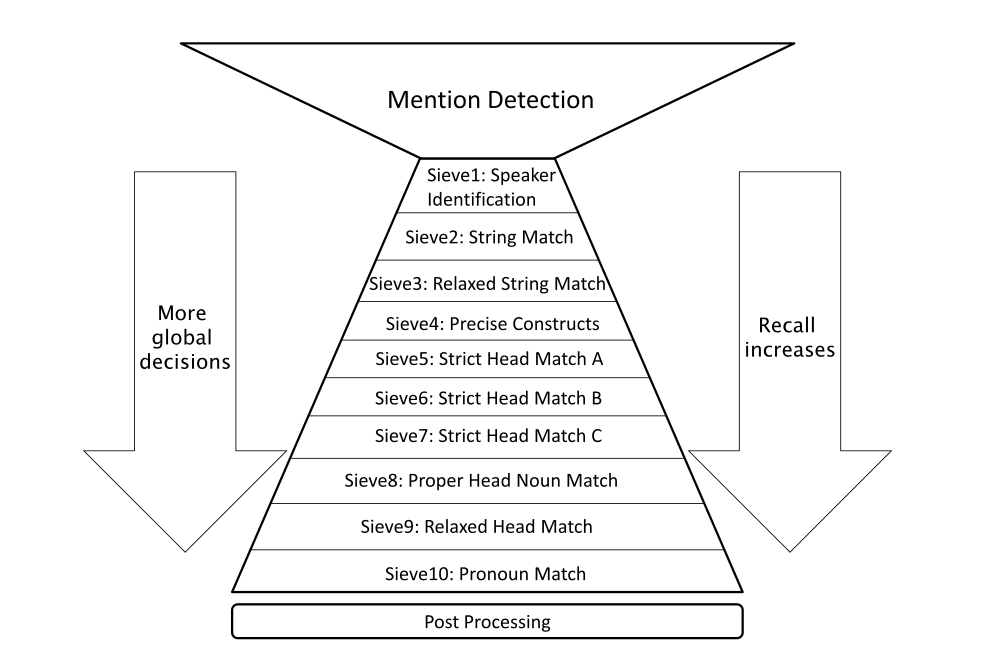
\includegraphics[scale=0.29]{stanford.png}
\end{frame}



\section{Module und Aufgaben}

\subsection{Module}

\subsection{Aufgaben}

\begin{frame}
\frametitle{Aufgabenverteilung}

bis 10.06.: Aufteilung der Pipeline 
\begin{itemize}
  \item \textit{DiscourseEntity}: Julian Baumann
  \item \textit{Sieve \& StringMatchSieve}: Xenia Kühling
  \item \textit{SieveDecoder}: Sebastian Ruder
\end{itemize}
ab 10.06.: Aufteilung der \textit{Sieves}
\begin{itemize}
  \item \textit{RelaxedStringMatchSieve}, \textit{PreciseConstructsSieve}, (\textit{SpeakerIdentificationSieve})
  \item \textit{StrictHeadMatch[ABC]Sieve}, \textit{RelaxedHeadMatch}
  \item \textit{ProperHeadNounMatch}, \textit{PronounMatch}
\end{itemize}

\end{frame}

\section{Zeitplan}

\begin{frame}

    \begin{gantt}{10}{9}
    \begin{ganttitle}
      \titleelement{Mai}{1}
      \titleelement{Juni}{4}
      \titleelement{Juli}{4}
    \end{ganttitle}
    \begin{ganttitle}
      \titleelement{27.05.}{1}
      \titleelement{03.06.}{1}
      \titleelement{10.06.}{1}
      \titleelement{17.06.}{1}
      \titleelement{24.06.}{1}      
      \titleelement{01.07.}{1}
      \titleelement{08.07.}{1}
      \titleelement{15.07.}{1}
      \titleelement{22.07.}{1}
    \end{ganttitle}
    \ganttbar{Pipeline läuft}{0}{2}
    \ganttmilestone[color=blue]{1. \textit{Sieve} läuft}{2}
    \ganttbar{\textit{Sieves} einfügen}{2}{3}
    \ganttmilestone[color=blue]{\textit{Sieves} laufen}{5}
    \ganttbar{Evaluation}{5}{2}
    \ganttbar[color=blue]{Bugfixes}{2}{5}
    \ganttbar{Präsentation}{7}{1}
    \ganttbar[color=blue]{Dokumentation}{5}{4}
  \end{gantt}
  
\end{frame}


\section{Softwarespezifikation}

\begin{frame}
\frametitle{Softwarespezifikation}

\begin{itemize}

	\item Datenformate
	\item Interfaces
	\item Datenstrukturen
	\item benötigte Ressourcen, verwendete Algorithmen

\end{itemize}

\end{frame}

\section{Quellen}


\end{document}